%%%%%%%%%%%%%%%%%%%%%%%%%%%%%%%%%%%%%%%%%
% Programming/Coding Assignment
% LaTeX Template
%
% This template has been downloaded from:
% http://www.latextemplates.com
%
% Original author:
% Ted Pavlic (http://www.tedpavlic.com)
%
% Note:
% The \lipsum[#] commands throughout this template generate dummy text
% to fill the template out. These commands should all be removed when 
% writing assignment content.
%
% This template uses a Perl script as an example snippet of code, most other
% languages are also usable. Configure them in the "CODE INCLUSION 
% CONFIGURATION" section.
%
%%%%%%%%%%%%%%%%%%%%%%%%%%%%%%%%%%%%%%%%%

%----------------------------------------------------------------------------------------
%	PACKAGES AND OTHER DOCUMENT CONFIGURATIONS
%----------------------------------------------------------------------------------------

\documentclass[12pt]{article}


\usepackage{fancyhdr} % Required for custom headers
\usepackage{lastpage} % Required to determine the last page for the footer
\usepackage{extramarks} % Required for headers and footers
\usepackage[usenames,dvipsnames]{color} % Required for custom colors
\usepackage{graphicx} % Required to insert images
\usepackage{subcaption}
\usepackage{listings} % Required for insertion of code
\usepackage{courier} % Required for the courier font
\usepackage{amsmath}
\usepackage{framed}

% Margins
\topmargin=-0.45in
\evensidemargin=0in
\oddsidemargin=0in
\textwidth=6.5in
\textheight=9.0in
\headsep=0.25in

\linespread{1.1} % Line spacing

% Set up the header and footer
\pagestyle{fancy}
\lhead{\hmwkAuthorName} % Top left header
\chead{\hmwkClass\ (\hmwkClassTime): \hmwkTitle} % Top center head
%\rhead{\firstxmark} % Top right header
\lfoot{\lastxmark} % Bottom left footer
\cfoot{} % Bottom center footer
\rfoot{Page\ \thepage\ of\ \protect\pageref{LastPage}} % Bottom right footer
\renewcommand\headrulewidth{0.4pt} % Size of the header rule
\renewcommand\footrulewidth{0.4pt} % Size of the footer rule

\setlength\parindent{0pt} % Removes all indentation from paragraphs

%----------------------------------------------------------------------------------------
%	CODE INCLUSION CONFIGURATION
%----------------------------------------------------------------------------------------

\definecolor{mygreen}{rgb}{0,0.6,0}
\definecolor{mygray}{rgb}{0.5,0.5,0.5}
\definecolor{mymauve}{rgb}{0.58,0,0.82}

\lstset{ %
  backgroundcolor=\color{white},   % choose the background color
  basicstyle=\footnotesize,        % size of fonts used for the code
  breaklines=true,                 % automatic line breaking only at whitespace
  captionpos=b,                    % sets the caption-position to bottom
  commentstyle=\color{mygreen},    % comment style
  escapeinside={\%*}{*)},          % if you want to add LaTeX within your code
  keywordstyle=\color{blue},       % keyword style
  stringstyle=\color{mymauve},     % string literal style
}

%----------------------------------------------------------------------------------------
%	DOCUMENT STRUCTURE COMMANDS
%	Skip this unless you know what you're doing
%----------------------------------------------------------------------------------------

% Header and footer for when a page split occurs within a problem environment
\newcommand{\enterProblemHeader}[1]{
%\nobreak\extramarks{#1}{#1 continued on next page\ldots}\nobreak
%\nobreak\extramarks{#1 (continued)}{#1 continued on next page\ldots}\nobreak
}

% Header and footer for when a page split occurs between problem environments
\newcommand{\exitProblemHeader}[1]{
%\nobreak\extramarks{#1 (continued)}{#1 continued on next page\ldots}\nobreak
%\nobreak\extramarks{#1}{}\nobreak
}

\setcounter{secnumdepth}{0} % Removes default section numbers
\newcounter{homeworkProblemCounter} % Creates a counter to keep track of the number of problems
\setcounter{homeworkProblemCounter}{0}

\newcommand{\homeworkProblemName}{}
\newenvironment{homeworkProblem}[1][Problem \arabic{homeworkProblemCounter}]{ % Makes a new environment called homeworkProblem which takes 1 argument (custom name) but the default is "Problem #"
\stepcounter{homeworkProblemCounter} % Increase counter for number of problems
\renewcommand{\homeworkProblemName}{#1} % Assign \homeworkProblemName the name of the problem
\section{\homeworkProblemName} % Make a section in the document with the custom problem count
\enterProblemHeader{\homeworkProblemName} % Header and footer within the environment
}{
\exitProblemHeader{\homeworkProblemName} % Header and footer after the environment
}

\newcommand{\problemAnswer}[1]{ % Defines the problem answer command with the content as the only argument
\noindent\framebox[\columnwidth][c]{\begin{minipage}{0.98\columnwidth}#1\end{minipage}} % Makes the box around the problem answer and puts the content inside
}

\newcommand{\homeworkSectionName}{}
\newenvironment{homeworkSection}[1]{ % New environment for sections within homework problems, takes 1 argument - the name of the section
\renewcommand{\homeworkSectionName}{#1} % Assign \homeworkSectionName to the name of the section from the environment argument
\subsection{\homeworkSectionName} % Make a subsection with the custom name of the subsection
\enterProblemHeader{\homeworkProblemName\ [\homeworkSectionName]} % Header and footer within the environment
}{
\enterProblemHeader{\homeworkProblemName} % Header and footer after the environment
}

%----------------------------------------------------------------------------------------
%	NAME AND CLASS SECTION
%----------------------------------------------------------------------------------------

\newcommand{\hmwkTitle}{Assignment 2} % Assignment title
\newcommand{\hmwkDueDate}{Friday, Nov 2\textsuperscript{nd}, 2018} % Due date
\newcommand{\hmwkClass}{CSC336} % Course/class
\newcommand{\hmwkClassTime}{LEC 0101} % Class/lecture time
\newcommand{\hmwkAuthorName}{Zhongtian Ouyang} % Your name
\newcommand{\hmwkAuthorID}{1002341012} % Your name

%----------------------------------------------------------------------------------------
%	TITLE PAGE
%----------------------------------------------------------------------------------------

\title{
\vspace{2in}
\textmd{\textbf{\hmwkClass:\ \hmwkTitle}}\\
\normalsize\vspace{0.1in}\small{Due\ on\ \hmwkDueDate}\\
\vspace{0.1in}
\vspace{3in}
}

\author{\textbf{\hmwkAuthorName}\\ \textbf{\hmwkAuthorID}}

\date{} % Insert date here if you want it to appear below your name

%----------------------------------------------------------------------------------------

\begin{document}

\maketitle
\clearpage
%----------------------------------------------------------------------------------------
%	PROBLEM 1
%----------------------------------------------------------------------------------------

% To have just one problem per page, simply put a \clearpage after each problem
%\begin{figure}[h!]
%\centering
%\includegraphics[width=0.6\linewidth]{q10a.png}
%\label{fig:q10a}
%\end{figure}\\

\begin{homeworkProblem}
\noindent \textit{prove $||x||_2 \leq ||x||_1$}\\

Choose an arbitrary integer $n\geq1$ and an arbitrary $x \in R^n$

$$(||x||_2)^{2}=\sum_{i=1}^{N}|x_i|^2\leq\sum_{i=1}^{N}|x_i|^2+2\times \sum_{j=1}^{N}\sum_{k=1}^{j-1}|x_j||x_k|=\left(\sum_{i=1}^{N}|x_i|\right)^2 = (||x||_1)^2$$

Since $(||x||_2)^{2} \leq  (||x||_1)^2$,  $||x||_2 \leq ||x||_1$


\end{homeworkProblem}
%----------------------------------------------------------------------------------------
%	PROBLEM 2
%----------------------------------------------------------------------------------------

\begin{homeworkProblem}
\noindent \textit{Norm question}\\

It is possible for some $x, y \in R^2$ such that $||x||_1 >||y||_1$, $||x||_2 <||y||_2$. \\

For example:
$$ x = \begin{bmatrix}0.5 & 0.6\end{bmatrix}, \quad y = \begin{bmatrix}0 & 1\end{bmatrix}$$
$$||x||_1 = |0.5| + |0.6| = 1.1,\quad ||y||_1 = |0| + |1| = 1, \quad ||x||_1 > ||y||_1$$
$$||x||_2 = \sqrt{|0.5|^2 + |0.6|^2} = \sqrt{0.61},\quad ||y||_2 = \sqrt{|0|^2 + |1|^2} = 1,\quad ||x||_2 < ||y||_2$$

\end{homeworkProblem}
%----------------------------------------------------------------------------------------
%	PROBLEM 3
%----------------------------------------------------------------------------------------

\begin{homeworkProblem}
\noindent \textit{Prove $||Ax|| \leq ||A||\cdot||x||$}\\

To prove that  $||Ax||_v \leq ||A||_m\cdot||x||_v$ for all $x \in R^n$ and all real $n \times n$ matrix, if $||A||_m$ is subordinate to a vector norm, we do it in cases:\\
Case 1:\\
 x is the zero vector. Ax would also be a zero vector. $ ||Ax||_v = 0 \leq 0 = ||A||_m\cdot ||x||_v$\\
 Case 2:\\
 x is not a zero vector. Proving $||Ax||_v \leq ||A||_m\cdot||x||_v$ is the same as proving  $\frac{||Ax||_v}{||x||_v} \leq ||A||_m$
 $$\frac{||Ax||_v}{||x||_v} \leq \max_{x \neq 0} \frac{||Ax||_v}{||x||_v} = ||A||_m$$\\
 So $||Ax||_v \leq ||A||_m\cdot||x||_v$
 


\end{homeworkProblem}
\clearpage
%----------------------------------------------------------------------------------------
%	PROBLEM 4
%----------------------------------------------------------------------------------------

\begin{homeworkProblem}
\noindent \textit{Solve system of equations}\\
\\
Code:
\begin{framed}
\begin{lstlisting}[language=matlab]
A = zeros(13);
b = zeros(13,1);
alpha = sqrt(2)/2;

A(1,2) = 1; A(1,6) = -1;
A(2,3) = 1; b(2) = 10;
A(3,1) = alpha;A(3,4) = -1;A(3,5) = -alpha;
A(4,1) = alpha;A(4,3) = 1;A(4,5) = alpha;
A(5,4) = 1;A(5,8) = -1;
A(6,7) = 1;
A(7,5) = alpha;A(7,6) = 1;A(7,9) = -alpha;A(7,10) = -1;
A(8,5) = alpha;A(8,7) = 1;A(8,9) = alpha;b(8) = 15;
A(9,10) = 1;A(9,13) = -1;
A(10,11) = 1;b(10) = 20;
A(11,8) = 1;A(11,9) = alpha;A(11,12) = -alpha;
A(12,9) = alpha;A(12,11) = 1;A(12,12) = alpha;
A(13,13) = 1;A(13,12) = alpha;   

f = A\b;

for i = 1:13
    fprintf('f%d = %f\n', i, f(i))
end

condA = cond(A);
r = b - A * f;
relative_residual = norm(r)/norm(b);
bound = condA * relative_residual;

fprintf('The condition number is %e\n', condA);
fprintf('The relative residual is %e\n', relative_residual);
fprintf('The bound is %e\n', bound);
\end{lstlisting}
\end{framed}
Output:
\begin{framed}
\begin{lstlisting}[language=matlab]
f1 = -28.284271
f2 = 20.000000
f3 = 10.000000
f4 = -30.000000
f5 = 14.142136
f6 = 20.000000
f7 = 0.000000
f8 = -30.000000
f9 = 7.071068
f10 = 25.000000
f11 = 20.000000
f12 = -35.355339
f13 = 25.000000
The condition number is 1.041221e+01
The relative residual is 2.012275e-16
The bound is 2.095224e-15
\end{lstlisting}
\end{framed}

a)\\
The system is set up by first transfroming the functions to the form with all fi in left side and constant in the right side.\\
The solved value of f1 to f13 are displayed in the output.\\

b)\\
As we have shown in the lecture, given Af = b, compute $\hat{f}$, $r = b - A\hat{f}$.\\
$A\hat{f} = b - r = \hat{b}$\\
$\Delta b = r = b - \hat{b}$\\
$\Delta f =f - \hat{f}$\\
In previous lecture note, we have proved that:$\frac{||\Delta f||}{||f||} \leq cond(A) \cdot \frac{||\Delta b||}{||b||}$\\
So $\frac{||\Delta f||}{||f||} \leq cond(A) \cdot \frac{||r||}{||b||}$\\
We can bound the relative error $\frac{||f - \hat{f}||}{||f||}$ by $cond(A) \cdot \frac{||r||}{||b||}$\\
The code for calcuting the bound is in above code section. The value of the bound on $\frac{||f - \hat{f}||}{||f||}$ is 2.095224e-15



\end{homeworkProblem}
\clearpage
%----------------------------------------------------------------------------------------
%	PROBLEM 5
%----------------------------------------------------------------------------------------

\begin{homeworkProblem}
\noindent \textit{Hilbert Matrix}\\

Part 1)\\
Code:
\begin{framed}
\begin{lstlisting}[language=matlab]
fprintf('%4s   %12s\n', 'n', 'Error');
max = 15;
x = ones(max, 1);
for n = 1:max
    cur_x = x(1:n);
    H = hilb(n);
    b = H * cur_x;
    x_hat = H\b;
    error = norm(cur_x - x_hat, Inf)/norm(cur_x, Inf);
    fprintf("%4d   %12e\n", n, error);
end
\end{lstlisting}
\end{framed}
Output:
\begin{framed}
\begin{lstlisting}[language=matlab]
   n          Error
   1   0.000000e+00
   2   7.771561e-16
   3   7.438494e-15
   4   4.518608e-13
   5   4.000800e-12
   6   5.724005e-10
   7   2.018865e-08
   8   2.046369e-07
   9   1.208404e-05
  10   3.592619e-04
  11   5.105110e-04
  12   4.996064e-01
  13   2.979912e+00
  14   5.019723e+00
  15   1.507535e+01
\end{lstlisting}
\end{framed}
From the output, we can see that when $n \leq 12$, the relative error in the solution is smaller than 1. When $n > 12$,  the relative error in the solution is greater than 1.\\
\clearpage
Part 2)
\begin{framed}
\begin{lstlisting}[language=matlab]
ns = 2:13;
cond_logs = zeros(1,12);
for i=1:12
    n = i + 1;
    cond_logs(i) = log(cond(hilb(n)));
end
plot(ns,conds,"-o");
\end{lstlisting}
\end{framed}
\begin{figure}[h!]
\centering
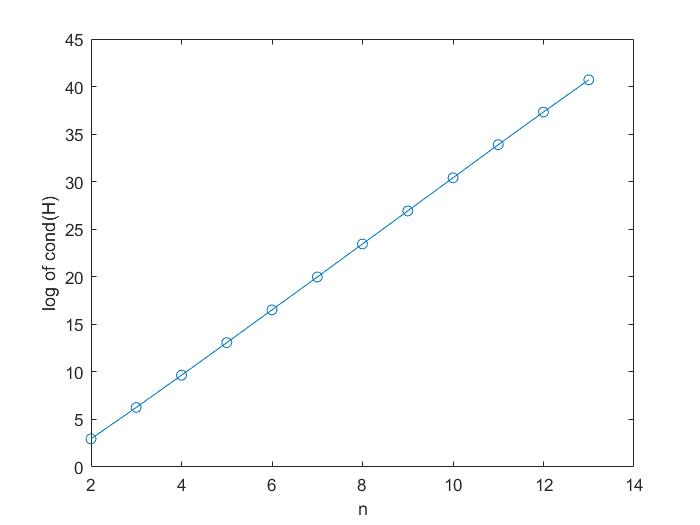
\includegraphics[width=0.6\linewidth]{Q5.jpg}
\label{fig:Q5}
\end{figure}
From the graph, we can see that the log of the condition number is in a roughly linear relationship with n. So condition number and n have a exponential relationship. If n is doubled, cond(H) is squared, etc.\\
Take two points from graph, say (2,2.9591) and (13, 40.7097), we can estimate the line by $log(cond(hilb(n))) \approx -3.9047 + 3.4319 \times n$\\
$cond(hilb(n)) \approx f(n) =  e^{-3.9047 + 3.4319 \times n}$\\

Part 3)
\begin{framed}
\begin{lstlisting}[language=matlab]
fprintf('%4s   %12s   %12s\n', 'n', 'Cond(H)', 'Max Error');
max_n = 15;
x = ones(max_n, 1);
for n = 1:max_n
    cur_x = x(1:n);
    H = hilb(n);
    b = H * cur_x;
    x_hat = H\b;
    fprintf("%4d   %12e   %12e\n", n, cond(H), max(abs(cur_x-x_hat)));
end
\end{lstlisting}
\end{framed}

\begin{framed}
\begin{lstlisting}[language=matlab]
   n        Cond(H)      Max Error
   1   1.000000e+00   0.000000e+00
   2   1.928147e+01   7.771561e-16
   3   5.240568e+02   7.438494e-15
   4   1.551374e+04   4.518608e-13
   5   4.766073e+05   4.000800e-12
   6   1.495106e+07   5.724005e-10
   7   4.753674e+08   2.018865e-08
   8   1.525758e+10   2.046369e-07
   9   4.931534e+11   1.208404e-05
  10   1.602503e+13   3.592619e-04
  11   5.220207e+14   5.105110e-04
  12   1.621164e+16   4.996064e-01
  13   4.786392e+17   2.979912e+00
  14   2.551499e+17   5.019723e+00
  15   2.495952e+17   1.507535e+01
\end{lstlisting}
\end{framed}

The `max error' row is the maximum absolute value of $x - \hat{x}$ at each value of n. \\
Since the components of x are all 1, we can easily observe the number of correct digits through this table. For example, if max error is 7.771561e-16, then we can know that at least the first 16 digits of any component in $\hat{x}$ is the same as the correspond component in x because the 17th digit is the first different digit.\\
With this logic, we can then see from the table that when cond(hilb(n)) is multiplied by about 10 times, the number of correct digits decrease by 1. And, suppose the condition number is $num \cdot 10^i$, the number of correct digits is roughly 17 - i.
\end{homeworkProblem}
\clearpage
%----------------------------------------------------------------------------------------

\end{document}
